\section{A ``hand-wavy'' first approach}

What we refer to as Artificial Intelligence is a broad 
collection of methods and techniques used to solve a variety
of problems that we collectively associate with ``human 
intelligence'', such as identifying and classifying images, 
processing natural language, and learning from data.  Roughly 
speaking, the discipline can be divided into the following 
sub-fields of research:

\begin{itemize}
	\item Neural Networks.
	\item Computer vision.
	\item Natural Language Processing.
	\item Speech processing.
	\item Machine Learning.
\end{itemize}

This work is concerned specifically with Machine Learning.  
Particularly with a subset of the field known as Reinforcement 
Learning. Some authors such as \cite{sutton2020reinforcement} 
divide the field of Machine Learning (ML) in three parts: 
supervised learning, unsupervised learning, and reinforcement 
learning.  Both supervised and unsupervised learning rely 
heavily on statistics-based techniques such as regression 
models and statistical inference. The techniques used in 
reinforcement learning (RL), rely on different models of what 
learning is, and tries to go beyond finding association rules 
for a simple, well-defined problem.

In contrast to supervised learning where a learning agent is 
given data labeled by a knowledgeable source and must ``learn'' 
to classify based on those initial labels, in unsupervised 
learning as well as reinforcement learning, there is no 
``training data'', the agent must act and optimize its strategy 
based only upon the reward or penalty resulting from making a 
certain decision. The key words here are \textit{optimize}, 
\textit{strategy} and \textit{decision}.

For a concrete example picture an android at a casino playing 
at a slot machine, only this machine has $k$ levers instead of 
just one.  This robot is instructed to win as much money as 
possible across some number of games. How could this be 
achieved? Surely each lever makes the machine operate 
differently and thus is more or less likely to get a jackpot. 
If this android were a person, the approach would probably be 
to, across many games, try each lever and see how much money 
comes out. Hopefully, after the first few games this human 
player has a clear idea of which are the best levers to pull. 
This too might be a good strategy for the robot to employ, so 
lets explore that idea further.

If you think about it, the slot machine analogy is not so 
different from the standard mental model we have of say an 
infant learning to crawl.  With poor vision and only its 
caretaker's voice as guide, it must learn to find its way to 
safety by trial and error. It cannot be given millions of 
examples of ``valid paths'' for extrapolation, as is the case 
with supervised learning. This agent learns by interacting with 
the environment itself.

In a certain sense RL leverages our intuitions about the nature 
of learning. All the main elements are there: cause and effect, 
goals, and consequences to decisions made, but as we will see, 
it also encodes more subtle concepts. For instance, delayed 
gratification and planning ahead. It also has the novelty of 
being goal-oriented rather than task-oriented as most Machine 
Learning techniques often are. For example, a self-driving car, 
``trained'' via supervised learning might train on millions of 
examples on what constitutes a valid steering wheel move, is
expected to extrapolate to situations outside the training 
data. Meanwhile a self-driving car, learning by being evaluated 
is learning how to drive as an activity consisting of hundreds 
of little tasks, all to be mastered simultaneously.

\section{Formalizing ideas}
Now, mathematically speaking, what does it \textit{mean} for a 
machine to ``learn''?

We might not get as far as what learning as a whole means for 
humans or machines, but we can certainly discuss what 
mechanisms allow self-driving cars to exist or computers to 
beat world champions of Chess and Go. For that, we need to 
identify the key concepts in the picture I painted and express 
them in the language of mathematics.

For now, we can gloss over the details of how might a machine 
make decisions, perceive goals, take actions or perceive 
rewards. Let us focus on one key component: the ``learning''. 
When we talk about the process of a machine learning something 
we are thinking about something or someone (referred to as 
agent henceforth) that is able to keep track of the decisions 
it made before and whether or not they resulted in positive 
results so it can later on apply that knowledge to become an 
increasingly better problem solver. If this agent is evaluated 
each time it carries out some task, we would like for its score 
to increase each successive time it tries to complete the task. 
The idea of a continuously improving score is the foundation of 
mathematical optimization.

\subsection{Optimization Theory}
As the name suggests, mathematical optimization is concerned 
with finding an ``optimal'' (whatever ``optimal'' means) 
solution to problems where an unambiguous score might be given 
to different solutions. Even if there is no best solution to a 
given problem, the techniques used in mathematical optimization 
often allow for a continuous improvement through iteration.

Going back to our slot machine example, each time the robot 
selects one of the $k$ levers the machine gives out a prize. 
The prizes vary greatly in size, and there is no way to know 
which ones give the biggest prizes in advance. Since the robot 
wants to maximize money earned, if one lever is consistently 
giving out bigger prizes it is likely to keep pulling it. The 
robot was rewarded earlier for choosing that lever by getting a 
big prize.  Similarly if a lever pull resulted in no prize at 
all, the robot lost money by playing and probably will not 
choose that lever again. In each iteration the player robot 
would like to increase more and more the prize, and is thus  
encouraged to keep track of which levers give good prizes, 
improving the average prize in each successive game.

We are now ready to peel away another layer of abstraction.  We 
now have an intuition of what it means for a machine to learn, 
or in other words continually improve. But in the model we 
discussed earlier, the player is making choices along the way. 
A predefined path is not programmed or even known. If it were 
known this would not be a problem at all, the robot could 
choose the known-good levers every single time. Since that is 
not the case the robot must choose and balance between 
exploring and exploiting the knowledge gained so far. What does 
it mean for this robot player to ``make choices''?

\subsection{Stochasticity}
Another key aspect we take for granted when we talk about 
machines learning is implicit in the word learning. If there 
were a predefined path for the robot to take we would hardly 
call that learning, it is merely reproducing instructions.  
What this means for us, is that we must allow for a framework 
in which our robots actions are not completely determined 
beforehand. In fancier words, the succession of events that 
determine the robots actions and responses to stimuli are not 
predetermined or \textit{deterministic}.

This idea is formalized through something called a 
\textit{stochastic process}. The word stochastic is just 
mathematical lingo for ``not entirely determined beforehand'' 
or ``aptly described as a random phenomenon''.  In particular, 
we can think of the robot as being in some state among quite a 
few possible. The robot can change states as time goes by but 
the transitions are not always the same and they do not 
necessarily carry the same reward or punishment.

For instance, the robot at the slot machine might have gotten a 
very big prize the first time it chose a certain lever but got 
almost nothing the next game. The feedback it got by choosing 
an action changes as time goes by, because the slot machine 
behaves randomly. This robot had a certain amount of 
information after pulling the lever for the first time: this is 
a good lever to pull. In the next game this robot already knows 
which lever might be a good bet, so among the $k$ possible 
options it might choose to pull the same lever as last time. 
Next time the reward is much smaller, the robot transitioned 
states in a sense. It was in a state were the best option was 
somewhat clear, to a state in which that one lever is no longer 
the most desirable option. It went from being certain to being 
forced to explore. We might think of this process a navigating 
the branches of a tree, making a decision every time a branch 
forks of into smaller branches.

[AQUI DIAGRAMA DE ARBOL]

\section{A slightly more nuanced example}
One of the major achievements and claims to fame for 
reinforcement learning in the past decades has been its use in 
some of the most famous matches in several classic board games.  
Chess was ``mastered'' when Kasparov, then chess grandmaster, 
was beaten by Deep Blue in 1997 \cite{silver2018chess}. Other 
board games with enormous state spaces such as Go, the game 
that originated in China, proved to be too complex for the 
techniques used by Deep Blue. Deep Blue was mainly based on 
hard-coded openings and endgames taken from other grandmaster 
games, which differs a lot from the RL approach. Go was much 
later attacked by another robot player named AlphaGo, developed 
by researchers from a company named DeepMind 
\cite{silver2017mastering}.  AlphaGo defeated Lee Sedol, the 
reigning human champion in 2016.  AlphaGo was one of the most 
notorious applications of RL and made the field even more 
popular. Since RL has proved to be very good for these kinds of 
tasks in the past, let us explore an example with a simpler 
board game.

\subsection{Duopoly, oligopoly, \ldots}
Consider a simplified version of a popular game whose name I 
avoid using as it might be copyrighted. This game consists of a 
circuit with predefined squares, some available for sale, in 
which a player is at any given moment. In order to move, a 
player spins an arrow fixed on the center of a circle that can 
stop at any of four circle segments numbered from 1 to 4. This 
is the number of squares the player moves forward. We refer to 
this spinning arrow as the \textit{spinner}.

You can find a scaled version of this game's board in figure 
\ref{fig:miniopoly-board}. The squares numbered 1 through 8 
(colored in shades of red, blue, purple and green) are 
available for purchase, while the white squares indicate a 
special action such as allowing the player to spin once more in 
the same turn, complete the circuit by going directly to the 
starting square and so on.

Going forward, picture a robot being ``trained'' to become a 
super player via the RL techniques we are slowly developing. At 
each turn the robot spins and moves forward however many 
squares the spinner indicates. If the robot lands on any square 
with a number on it, it might acquire that square for itself. 
From that moment on, if the opponent lands on that square the 
robot player will be paid rent. If the robot lands on that same 
square, it may build hotels on it so next time the opponent 
lands there, the rent payed will be much higher. The robot also 
receives money every time it completes the circuit.

As you might have guessed, the point of the game is to make the 
most amount of money. The game ends when either the robot or 
it's opponent go bankrupt. What purchase strategy must the 
robot follow to win?
\begin{figure}[h]
	\centering
	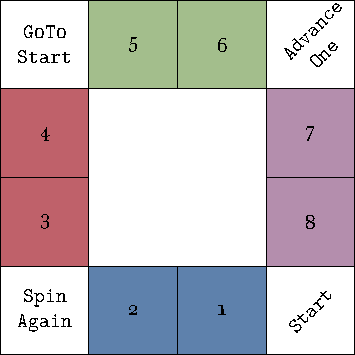
\includegraphics[width=.65\textwidth]{img/board.pdf}
	\caption{Board for the game described earlier.}
	\label{fig:miniopoly-board}
\end{figure}

First off, unlike the slot machine-playing robot, this robot 
player cannot entirely choose which square to move to, it can 
only decide if it wants to purchase it or not once it has 
landed on it. The biggest number it can spin is 4, and even if 
it got to spin again the furthest it could go is square 5. Even 
if the robot wanted to go to square number 8 and buy it, there 
is no possible way to do that.

Figure \ref{fig:miniopoly-diagram-start} shows a simplified 
version of the board. Only the squares accessible on the first 
turn are shown, along with arrows indicating the possible 
transitions between the starting square and the rest.
\begin{figure}[h]
	\centering
	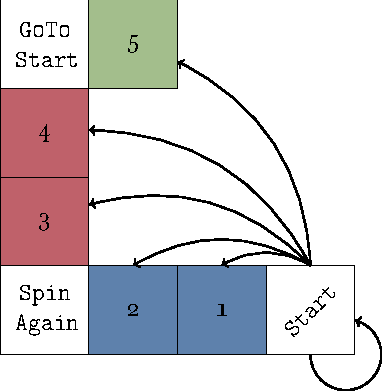
\includegraphics[width=.65\textwidth]{img/diagram-start.pdf}
	\caption{Squares accessible on the first turn.}
	\label{fig:miniopoly-diagram-start}
\end{figure}

In figure \ref{fig:miniopoly-diagram-start} we can see all the 
possible squares the robot might land on and then buy starting 
from the first turn. Notice how squares 6 and further are not 
included. If the robot were to spin a 4, the red square with 
number 3 is the furthest it could go. If it were to land on 
\texttt{Spin Again} and then spin a 4, the largest possible 
spin, it could move four squares: from \texttt{Spin Again} to 
3, then to 4, then to \texttt{Goto Start}, and finally to 
square 5, exhausting its possible moves.

Notice how in this figure we only care about the starting and 
ending points, not the transit points, so that is why there are 
no arrows pointing to the squares that move the player 
elsewhere like \texttt{Spin Again} and \texttt{Goto Start}. 
This is the reason there is an arrow that points from 
\texttt{Start} to itself. This transition might happen. In 
fact, we know what it takes for this to happen: land on 
\texttt{Spin Again}, and then land on \texttt{Goto Start}. In 
other words, this transition happens if the robot spins a 3 two 
consecutive times.

If the robot were to land on \texttt{Spin Again}, then spin a 
3, it would ``land'' on \texttt{Goto Start}, finishing its turn 
back at the starting square. That particular move results in 
the robot going back to the start and getting paid for 
completing the circuit, without running the risk of landing on 
a square someone else owns. That sounds like a very desirable 
move (for us looking at the big picture, the robot cannot see 
that far ahead yet). Since we would like this to happen, we 
might ask how likely is for that to happen.

\begin{figure}[h]
	\centering
	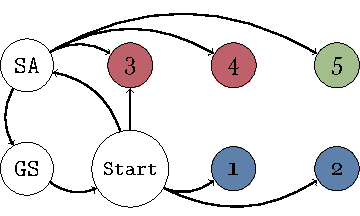
\includegraphics[width=\textwidth]{img/transicion.pdf}
	\caption{Diagram showing the possible transitions to the 
	numbered squares, starting the turn at \texttt{Start}. 
	Squares \texttt{GoTo Start} and \texttt{Spin Again} are 
	abbreviated as \texttt{GS} and \texttt{SA} respectively.}
	\label{fig:miniopoly-transicion}
\end{figure}

Lets try to analyze how likely the robot is to end up in this 
particularly rewarding situation. For that it's often helpful 
to think of the possible steps that lead to it. On figure 
\ref{fig:miniopoly-transicion} we can see a more abstract 
diagram of the possible movements the robot might make, and 
this time we are taking into account intermediate squares. Each 
arrow represents where the robot might land after spinning, not 
necessarily it's final resting square. Now, using some very 
basic probability theory we can calculate how likely it is for 
the robot to ``take that route'' so to speak. Once we do, we 
can calculate how likely a ``route'' or sequence of arrows is.

\begin{figure}[h]
	\centering
	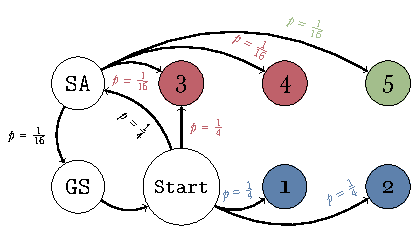
\includegraphics[width=\textwidth]{img/transicion-markov.pdf}
	\caption{Transition diagram with transition probabilities}
	\label{fig:miniopoly-transicion-markov}
\end{figure}

At the moment it is not important why some arrows have certain 
probabilities, and some might not be terribly obvious even for 
someone acquainted with some basic probability. In figure 
\ref{fig:miniopoly-transicion-markov} to find the probability 
of getting to a certain square (say 6 for example) we look only 
at the last arrow, as it takes into account the probability of 
the previous step happening. For example, the probability of 
the move that takes the player from \texttt{Start} back to 
\texttt{Start} we can look at the bottom left corner of figure 
\ref{fig:miniopoly-transicion-markov}. The player moves to 
\texttt{Spin Again} with probability 1/4 because the spinner 
has an equal chance of making the player move either 1, 2, 3 or 
4 squares. Once the player is on \texttt{Spin Again} and spins 
once more, it has a chance of 1/16 of landing on \texttt{GoTo 
Start}. The final arrow pointing from \texttt{GoTo Start} to 
\texttt{Start} is not annotated with the probability of it 
happening, since that transition is not random. Once the player 
lands there, the next thing that happens to the player is 
always the same: go to the starting square.

The robot we are trying to teach moves as the figure above 
suggests. There is a different diagram for each square in which 
the player finds itself at the start of its turn. The robot is 
not aware of this, all it knows is that it spins, and then is 
transported elsewhere and must decide whether to buy or not (if 
the square is available). All it knows is it's current 
position, and the gains or losses it sustained on the other 
squares it has visited. Crucially, landing on a square 
previously visited does not necessarily mean the reward will be 
the same as last time. For instance, if it lands on square 3 
and decides not to buy it, the reward was a net 0, but the 
other player may buy it so that the next time the robot visits 
that square it has to pay rent, which would mean a loss. Also, 
the reward for buying a square may come much later on or not at 
all. This robot must somehow keep track of what the expected 
reward for landing somewhere might be, recording it somewhere 
and tallying up as it goes.

For instance after a few turns it might have something fig. 
\ref{fig:hist-miniopoly} on its head to help make decisions.

After playing a few games, keeping a record of which squares it 
bought, the player might make a graph to discover what moves it 
made that resulted in higher rewards at the end of the game. 
Such a graph might look like figure \ref{fig:hist-miniopoly}, 
which is a violin plot. In this plot, a violin-shaped figure 
gives the robot an idea of what squares yielded better rewards 
or smaller losses when bought or when left for other players to 
buy. The height of the violin indicates how high the reward was 
at the end of the game, while the width of the violin helps the 
robot decide whether that outcome was a fluke or not. A thin 
violin at a specific height (reward) indicates that over the 
games it has played so far, that specific reward marked by the 
y-axis is not as common as the reward that corresponds to the 
thicker parts of the violin.
% Se entiende??

\begin{figure}
\centering
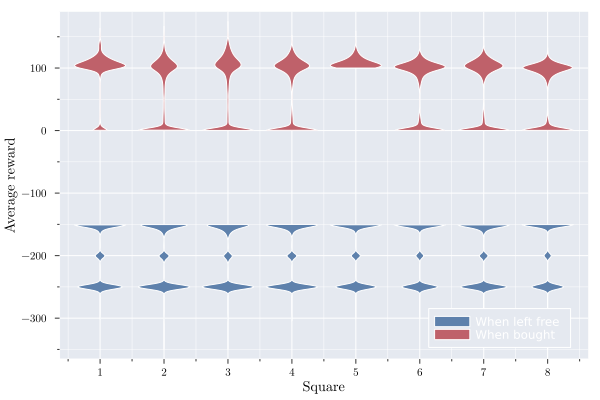
\includegraphics[width=\textwidth]{img/hist-miniopoly.tikz}
\label{fig:hist-miniopoly}
\caption{Violinplot of the average reward obtained at the end 
of the game by buying or not buying a square.}
\end{figure}

This figure was created by simulating 20 thousand 
games\footnote{The entire simulation took around 70 seconds.} 
and recording what rewards the robot player obtained at the end 
of the game by buying or not buying a certain square. For 
instance, if it bought square 3, the record shows the initial 
loss of however much money the player paid for the square. 
Later on in the game if the opponent lands on square 3 and pays 
rent, that rent is recorded as a gain for the robot player. 
That number is averaged out at the end of the game so the robot 
can analyze this information later. One way of analyzing this 
information to improve strategy is precisely to make a graph 
like the one in figure \ref{fig:hist-miniopoly}

Its stands to reason that as this graph is updated the learning 
agent will be able to make progressively better choices by 
identifying the patterns. For instance, it might notice from 
figure \ref{fig:hist-miniopoly} that buying square number 5 
consistently results in higher rewards at the end of the game. 
The robot noticed this because the violin corresponding to 
square 5 is noticeably higher than the others. Simple as this 
example might be, the essence is similar to the powerful 
programs that defeat world champions of chess and Go.

This example covers most of the core ideas of what is referred 
to as the Reinforcement Learning Problem. We will explore the 
ideas presented here in much more detail along this thesis and 
crucially, focus on something we left out on this example. How 
can a purchase strategy be improved upon?

\section{Wrapping up}
So far we have developed a mental model of what to do should we 
wish to teach a robot how to drive or beat a world champion of 
Go. The rest of this thesis is dedicated to the careful 
development of the ideas here presented into the language of 
mathematics. Specifically, tackling questions such as:
\begin{itemize}
	\item What mechanism allows the robot player to learn from 
	experience and fine-tune it's strategy to become better?
	\item How can we tell when a new strategy is better than an 
	old one?
	\item Is it possible to find \textit{the} best strategy? 
	How difficult is it?
\end{itemize}

Beyond mere description, this exercise has the potential to 
unlock \textit{insight}. As is often said by legendary math 
communicator Grant Sanderson\footnote{From the YouTube channel 
\href{https://www.youtube.com/channel/UCYO_jab_esuFRV4b17AJtAw}{3blue1brown}}(loose 
quote), the point in formulating things this way is to gain a 
deeper understanding of the phenomenon. So let's dive right in.
